% Compile with XeLaTeX or LuaLaTeX
\documentclass{article}
\usepackage[paperwidth=16cm, paperheight=24cm, margin=0pt]{geometry}
\usepackage{graphicx}
\usepackage{tikz}
\usepackage{fontspec}
\usepackage{xcolor}

% Define fonts (using standard Latin Modern Sans, widely available)
\setsansfont{Latin Modern Sans}
\newfontfamily\titlefont{Latin Modern Sans}[LetterSpace=12]

\begin{document}
\pagestyle{empty} % No page numbers

% 1. Background Image Layer
\begin{tikzpicture}[remember picture, overlay]
    % Place the background image edge-to-edge.
    % IMPORTANT: Rename your generated background image to "cover_background.png"
    % and place it in the same folder as this .tex file.
    \node[inner sep=0pt, outer sep=0pt, anchor=center] at (current page.center) {
        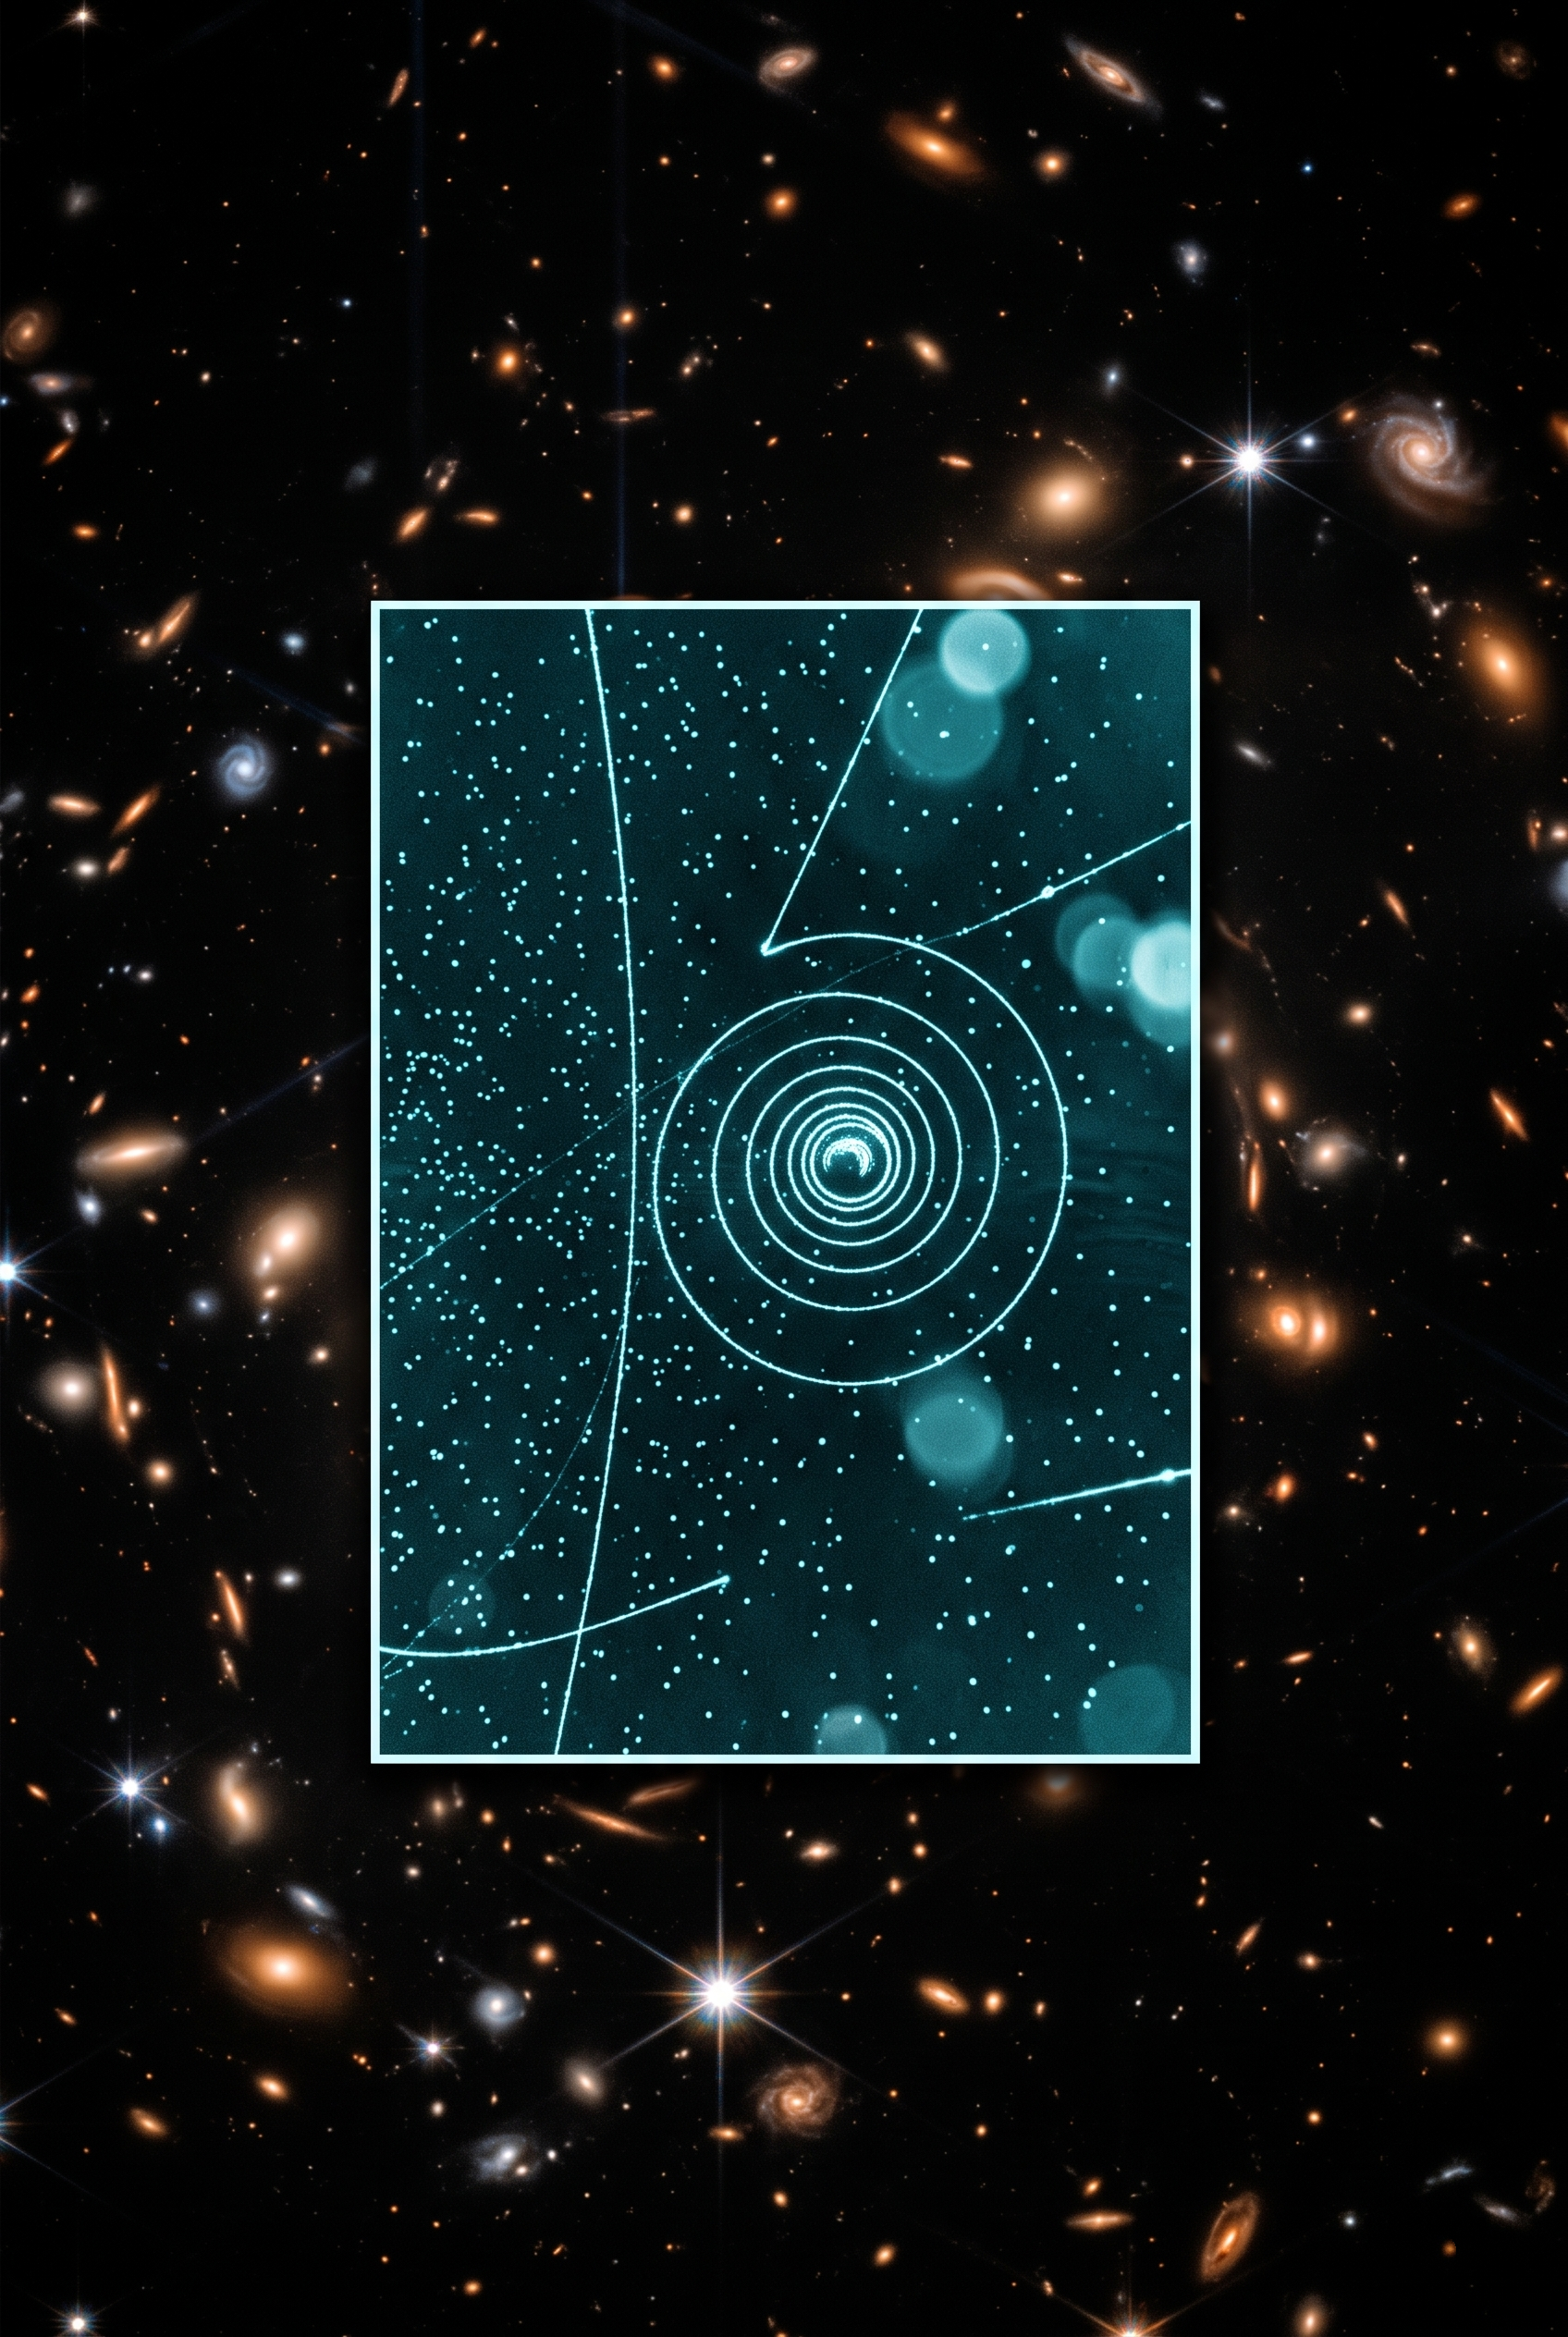
\includegraphics[width=\paperwidth, height=\paperheight]{kapak01.png}
    };
\end{tikzpicture}

% 2. Text Overlay Layer
\begin{tikzpicture}[remember picture, overlay]

    % ==========================================
    % TOP SECTION: TITLE & SUBTITLE
    % ==========================================
    % Title positioned 3.5 cm from the top edge
    \node[anchor=north, text=white, align=center] at ([yshift=-3.5cm]current page.north) {
        \titlefont\fontsize{32}{38}\bfseries\selectfont KUANTUM FİZİĞİ
    };

%    % Subtitle positioned 5.5 cm from the top edge
%    \node[anchor=north, text=cyan!20!white, align=center] at ([yshift=-5.5cm]current page.north) {
%        \sffamily\fontsize{16}{20}\selectfont Akdeniz Üniversitesi
%        %Lisans Düzeyinde Giriş
%    };

    % ==========================================
    % BOTTOM SECTION: AUTHOR & CAPTION
    % ==========================================
    % Author positioned 4.5 cm from the bottom edge
    \node[anchor=south, text=white, align=center] at ([yshift=4.5cm]current page.south) {
        \sffamily\fontsize{18}{22}\selectfont Mesut Karakoç
    };

    % Dark semi-transparent rectangle for caption legibility
    % Spans the entire width of the page, 2 cm high from the bottom edge
    \fill[black, opacity=0.75] (current page.south west) rectangle ([yshift=2cm]current page.south east);

    % Caption text positioned 0.7 cm from the bottom edge
%    \node[anchor=south, text=white!85, align=center, text width=14cm] at ([yshift=0.7cm]current page.south) {
%        \sffamily\fontsize{9}{12}\itshape\selectfont 
%        Kapak görseli: CERN Gargamelle kabarcık odasında 1973'te gözlenen leptonik \\
%        olaydan esinlenilmiştir. % Ayrıntı için bkz. Kapak Üzerine.
%    };


    % --- ALT BLOK ZEMİNİ (arka plan yeterince koyuysa bu satırları silin) ---
    \fill[black, opacity=0.50]
    (current page.south west) rectangle
    ([yshift=3.3cm]current page.south east);
    
    % --- AYET: alttan 1.95 cm ---
    \node[anchor=south, text=white!88, align=center, text width=12.2cm]
    at ([yshift=1.95cm]current page.south)
    {\itshape\fontsize{8.5}{12}\selectfont
    	“\,…Ne yerde ne de gökte, zerre miktarı bir şey bile rabbinin bilgisi
    	dışında kalmaz; bundan daha küçük veya daha büyük ne varsa istisnasız
    	apaçık bir kitapta yazılıdır.\,”};
    
    % --- AYET KÜNYESİ: alttan 1.55 cm ---
    \node[anchor=south, text=cyan!35!white, align=center]
    at ([yshift=1.55cm]current page.south)
    {\fontsize{7}{9}\selectfont Yûnus, 10/61};
    
    % --- AYRAÇ ÇİZGİ: alttan 1.22 cm ---
    \draw[white, opacity=0.35, line width=0.4pt]
    ([yshift=1.50cm, xshift=-1.6cm]current page.south)
    -- ([yshift=1.50cm, xshift=1.6cm]current page.south);
    
    % --- YAZARIN CÜMLESİ: alttan 0.55 cm ---
    \node[anchor=south, text=white!92, align=center, text width=12.2cm]
    at ([yshift=0.55cm]current page.south)
    {\fontsize{8.5}{12}\selectfont
    	Milyarlarca ışık yılından tek bir elektronun izine —\\
        	bu ölçeklerin tamamı fiziğin konusudur.};


\end{tikzpicture}
\end{document}
```http://googleusercontent.com/image_generation_content/777